\chapter{Properties of Single-Wall Carbon Nanotubes}

The properties of carbon nanotubes (CNT) strongly depend on their crystal structure. CNTs consists of carbon atoms bound together via sp$^2$ orbitals ($\sigma$ bonds) and arranged in a honeycomb lattice \cite{soavi2016ultrafast}. Due to the similarities between the crystal structures of graphene and CNTs, different CNT species can be classified using the basis vectors of the graphene lattice \cite{charlier2007electronic}. In fact, the countless ways of rolling up a graphene sheet into a nanotube evince that CNTs can exhibit varying helical geometries and symmetries with respect to their axial direction as shown in Figure \ref{fig:symmetries}. 

\begin{figure}[h]
	\centering
	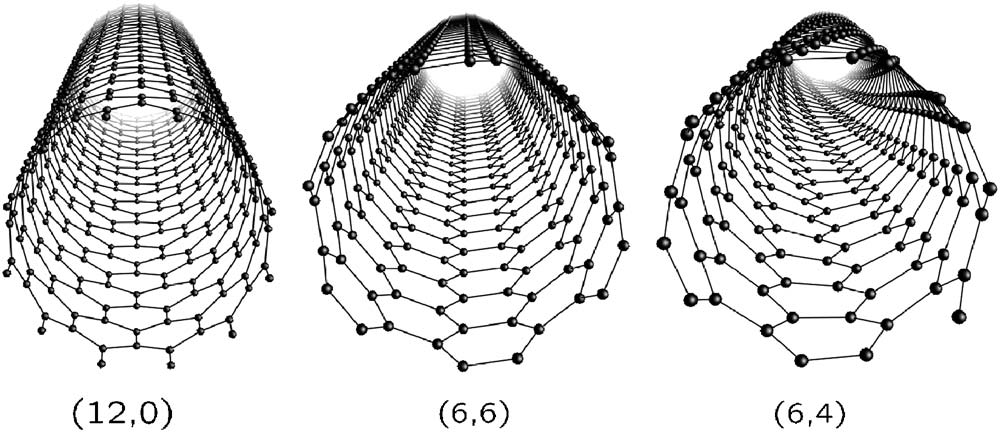
\includegraphics[scale=0.4]{images/chapter_optical_props/nanotube_symmetries_charlier}
	\caption{Crystal structures of (12,0), (6,6) and (6,4) single-wall carbon nanotubes. Reproduced from Ref \cite{charlier2007electronic}.}
	\label{fig:symmetries}
\end{figure}

These morphological properties dictate the allowed electronic states by asserting boundary conditions on the electron wavefunction along the circumferential direction \cite{charlier2007electronic}. These allowed states exhibit anisotropic features and obey a set of optical selection rules that govern allowed inter-band transitions. Moreover, the effect of strong electron-electron interactions impose further modifications to the electronic structure and effectively suppress the presence of any free-electron continuum states \cite{ando1997excitons}. This unusual behavior alone distinguishes carbon nanotubes from conventional semiconductors as they typically exhibit relatively weak Coulomb interactions \cite{ando1997excitons}.



\section{Crystal Structure of Carbon Nanotubes}

\subsection{Definition of the Chiral Vector $\vec{C_h}$}

Each unique species of carbon nanotubes can be	 denoted using a set of indices ($m$,$n$). These integers $m$ and $n$ define the chiral vector $\vec{C_h }$ expressed as 
\begin{equation}
	\vec{C_h} = n {\vec{a_1}} + m {\vec{a_2}} \equiv (m,n)
	\label{eq:chiral_vec}
\end{equation}

where $\vec{a_1}$ and $\vec{a_2}$ represent the lattice basis vectors of the 2D graphene sheet as shown in Figure \ref{fig:chiral_vectors} \cite{nanot2013single}. This chiral vector $\vec{C_h}$ yields the nanotube diameter $d_t$ via the expression

\begin{equation}
	d_t = \dfrac{|\vec{C_h}|}{\pi} = \dfrac{a_{C-C}}{\pi}\sqrt{3(m^2 + mn + n^2)},
\end{equation} 

where $a_{C-C} \approx$ \SI{1.44}{\angstrom} defines the nearest-neighbor distance between carbon atoms in graphene \cite{nanot2013single}.  

\begin{figure}[ht]
	\centering
	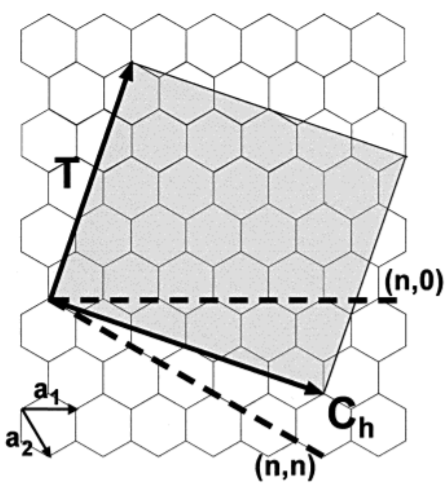
\includegraphics[scale=1]{images/chapter_optical_props/chiral_vectors_sheet.png}
	\caption{{\color{red}UNFINISHED CAPTION}}
	\label{fig:chiral_vectors}
\end{figure}

\subsection{Chiralities of Semiconducting and Metallic Nanotubes}
The chiral vector $\vec{C_h}$ also provides the means of distinguishing between semiconducting and metallic nanotubes. Furthermore, the variable $\nu$ defined as 
\begin{equation}
	\nu \equiv (n-m) \mathrm{\hspace{1.5mm} mod \hspace{1.5mm}} 3,
	\label{eq:nu_cnt}
\end{equation}
is also used to label different nanotubes. In general, $(n,n)$ carbon nanotubes, also commonly referred to as ``armchair'' nanotubes, constitute the set of all metallic nanotubes \cite{nanot2012optoelectronic}. All $(n,m)$ nanotubes where $n-m = 3j$ ($j > 0$) comprise the set of small-gap ($\sim1 - 100$ meV band gap energy) semiconductors \cite{nanot2012optoelectronic}. These first two classes satisfy the condition that $\nu = 0 $. The remaining nanotubes outside of these two categories include medium-gap semiconductors ($\sim0.5 - 1$ eV band gap energy) \cite{nanot2012optoelectronic}. For these CNTs, $\nu = \pm 1$.


\section{Optical and Electronic Properties}

\subsection{Electronic Band Structure}

Given the similarities between CNTs and graphene, calculating the electoronic band structure of graphene is the first step towards determining that of CNTs. A simple tight-binding model can be used to calculate the band structure of graphene. Such a model includes first nearest-neighbor interactions involving the $\pi$-orbitals of two atomic sites located at positions and $\vec{a_1}$ as well as $\vec{a_2}$ \cite{charlier2007electronic}. Here, $\vec{a_1}$ and $\vec{a_2}$ represent the lattice vectors of graphene. Furthermore, a hopping term $\gamma_0 \approx 2.9$ eV  characterizes the interactions between neighboring $\pi$-orbitals \cite{charlier2007electronic}. The Hamiltonian $\mathcal{H}$ for this simple system is then written as 

\begin{figure}[h]
	\centering
	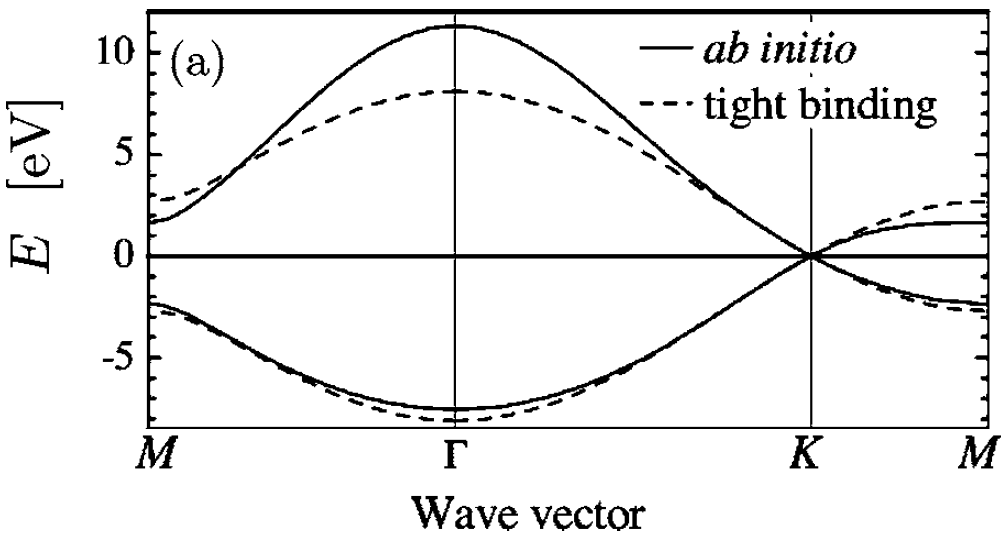
\includegraphics[scale=0.5]{images/chapter_optical_props/graphene_band_charlier}
	\caption{Electronic band structure of graphene determined using a tight-binding model (dashed line) and through ab-initio calculations (solid line). Reproduced and modified from Ref \cite{reich2002tight}.}
	\label{fig:graphene_band}
\end{figure}


\begin{equation}
	\mathcal{H} = \begin{bmatrix} 
	0 & \alpha(k) \\
	\alpha^*(k) & 0
	\end{bmatrix}
\end{equation}

where $\alpha(\vec{k}) = (1 + e^{-i \vec{k}\cdot \vec{a_1}} + e^{-i \vec{k}\cdot \vec{a_2}})$ and $\alpha^*(\vec{k})$ refers to the complex conjugate of $\alpha(\vec{k})$\cite{charlier2007electronic}. In addition, $\vec{k}$ stands for a reciprocal space vector within the first Brillouin zone. Diagonalizing this matrix yields the energy dispersion 

\begin{equation}
	E^{\pm} (k_x, k_y) = \pm \gamma_0 \sqrt{1 + 4 \cos\dfrac{\sqrt{3}k_x a}{2}\cos\dfrac{k_y a}{2} + 4 \cos^2 \dfrac{k_y a}{2}}.
	\label{eq:graphene_band}
\end{equation} 

 Here, $E^-$ and $E^+$ stand for the dispersion relations of the valence and conduction bands respectively. The variables $k_x$ and $k_y$ denote the x- and y-components of $\vec{k}$. Moreover, the constant $a = \sqrt{3}a_{C-C}$, where $a_{C-C} \approx$ \SI{1.44}{\angstrom} and refers to the nearest-neighbor distance between the lattice sites. 

Figure \ref{fig:graphene_band} presents a plot of Eq. \ref{eq:graphene_band} as compared with a band structure calculation using ab-initio methods. Despite the disagreement between both approaches, they both predict a linear dispersion in the region near the K point \cite{charlier2007electronic}. This region of the band structure is commonly referred to as the Dirac cone	\cite{charlier2007electronic}. Moreover, both models identify graphene as a metal since the valence and conduction bands intersect at this K point position \cite{charlier2007electronic}. In conjunction with the band structure of graphene, the so-called zone-folding approximation yields the band structure of CNTs. 


\begin{figure}[h]
	\centering
	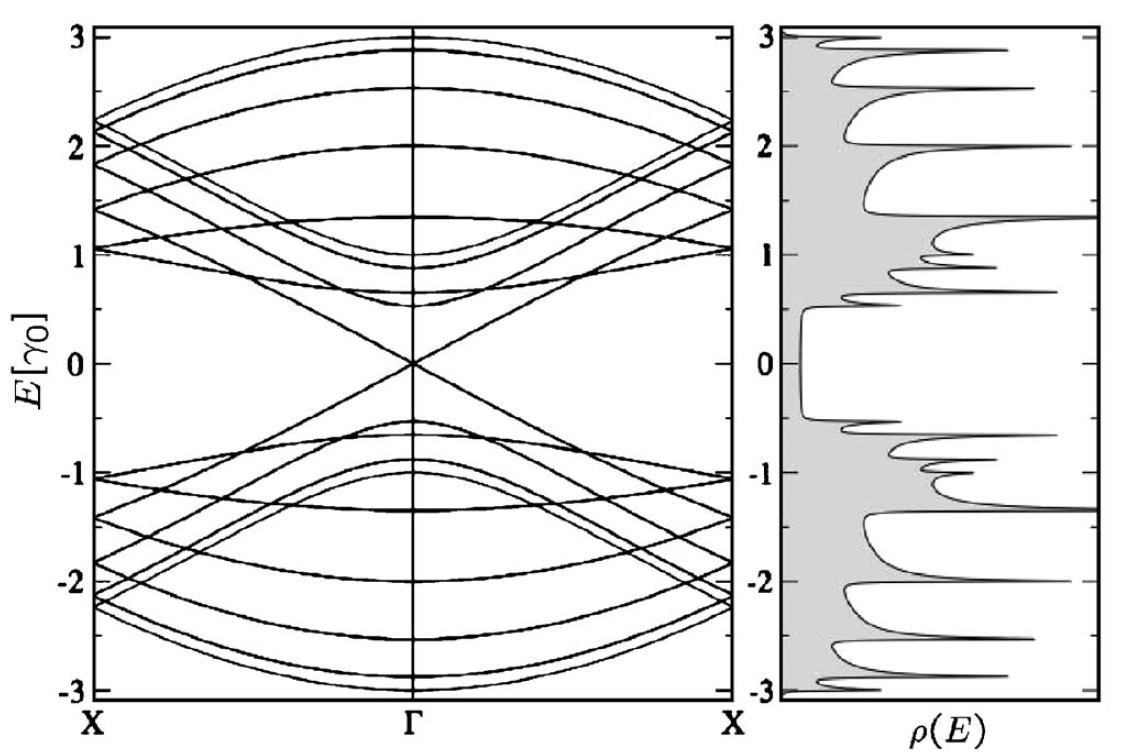
\includegraphics[scale=0.36]{images/chapter_optical_props/nine_zero_band_charlier}
	\caption{Band structure and density of states for a (9,0) carbon nanotube derived using the zone-folding scheme. These are plotted in units of $\gamma_0 \approx 2.9$, the tight-binding hopping energy between first nearest-neighbors. Reproduced from \cite{charlier2007electronic}.}
	\label{fig:nine_zero_cnt}
\end{figure}

The zone-folding method asserts that the periodic boundary conditions along the circumferential direction of CNTs dictate the quantization of the allowed $\vec{k}$ vectors in the electronic band structure \cite{charlier2007electronic}. This condition applied to the electron wavefunction $\Psi(\vec{r})$ is expressed as 
\begin{equation}
 \Psi_{\vec{k}}(\vec{r} + \vec{C_h}) = e^{i \vec{k} \cdot \vec{C_h}} \Psi_{\vec{k}}(\vec{r}) = \Psi_{\vec{k}}(\vec{r}),
 \label{eq:boundary_cond}
\end{equation}
where $\vec{r}$ and $\vec{k}$ respectively define vectors in real and reciprocal space on the surface of the CNT \cite{charlier2007electronic}. Furthermore, $\vec{C_h}$ represents the chiral vector defined in Eq. \ref{eq:chiral_vec}. 

Equation \ref{eq:boundary_cond} reveals that the symmetry of the CNT given by the chirality $\vec{C_h} \equiv (n,m)$ determines the band structure. Figures \ref{fig:nine_zero_cnt} and \ref{fig:ten_zero_cnt} illustrate this point. The band structure of nanotubes for which $\nu = 0$ include the Dirac cone along with additional sub-bands within the valence and conduction bands. These include the set of armchair nanotubes ($n=m$) that are metallic (gapless) \cite{nanot2012optoelectronic}. Although non-armchair nanotubes ($n\neq m$) also fit into the $\nu = 0$ category, these exhibit so-called curvature-induced band gaps and behave as narrow-gap semiconductors \cite{nanot2012optoelectronic}.  Whereas, the band structures of semiconducting nanotubes for whom $\nu = \pm 1$ exclude the presence of a Dirac cone \cite{charlier2007electronic}.
 
%\begin{figure}[h]
%	\centering
%	\begin{subfigure}{0.45\textwidth}
%		\centering
%		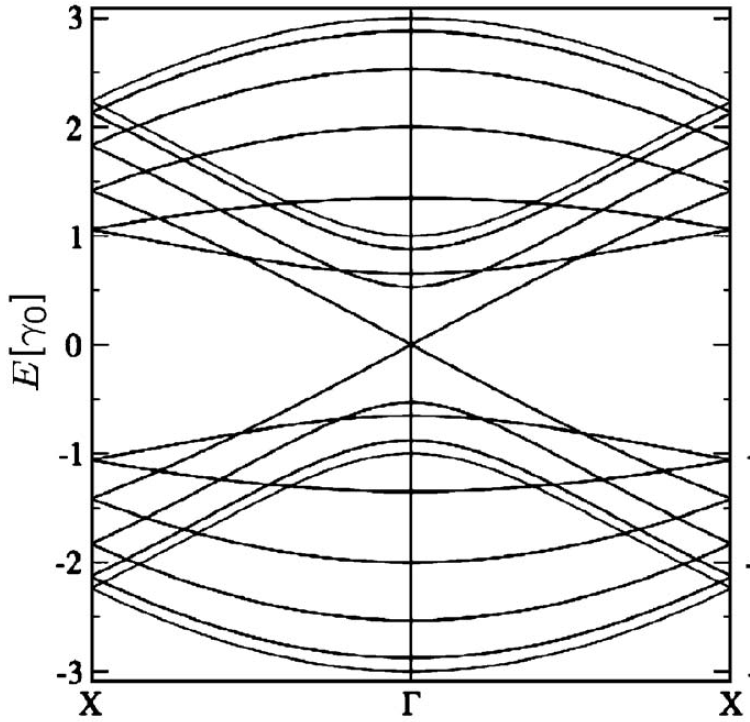
\includegraphics[scale=0.36]{images/chapter_optical_props/nine_zero_band_charlier_2}
%		\caption{Metallic}
%	\end{subfigure}
%	\qquad
%	\begin{subfigure}{0.45\textwidth}
%		\centering
%		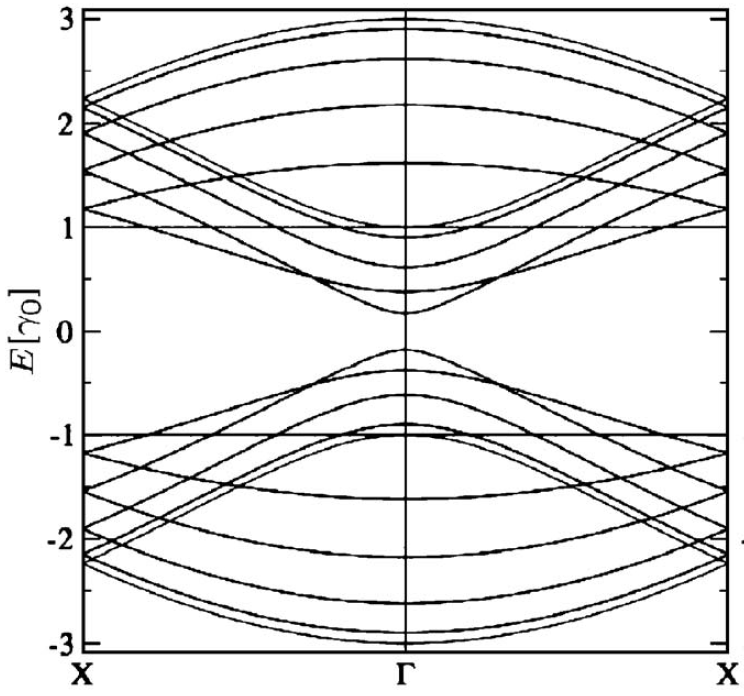
\includegraphics[scale=0.38]{images/chapter_optical_props/ten_zero_band_charlier_2}
%		\caption{Metallic}
%	\end{subfigure}
%	\caption{Reproduced and modified from Ref \cite{charlier2007electronic}.}
%\end{figure}


\begin{figure}[h]
	\centering
	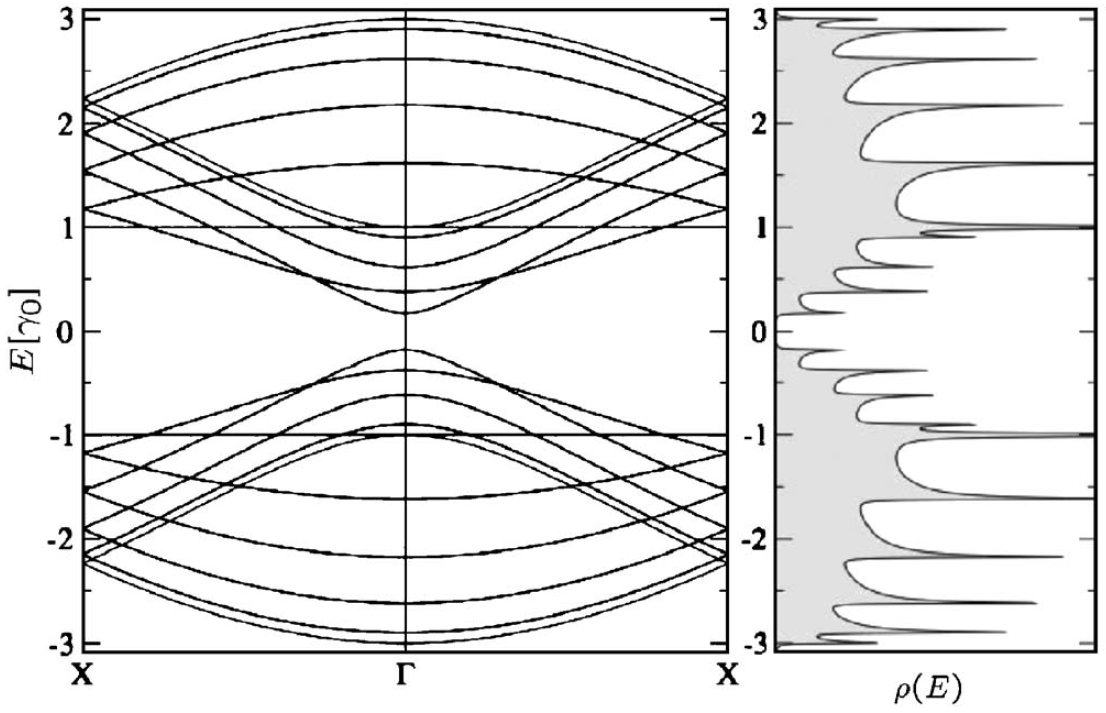
\includegraphics[scale=0.38]{images/chapter_optical_props/ten_zero_band_charlier}
	\caption{Band structure and density of states for a (10,0) carbon nanotube derived using the zone-folding scheme. These are plotted in units of $\gamma_0 \approx 2.9$ which represents the tight-binding hopping energy between first nearest-neighbors. Reproduced from \cite{charlier2007electronic}.}
	\label{fig:ten_zero_cnt}
\end{figure}


\subsection{Optical Selection Rules}

Selection rules dictate the optical transitions that can occur. Such optical processes depend upon the conservation of both energy and angular momentum \cite{weismanKonoBook}. The notation E$_{ij}$ denotes an inter-band transition between the valence sub-band $i$ and the conduction sub-band $j$ \cite{weismanKonoBook}. In addition, $\Delta n \equiv i - j$ defines the difference between the band indices $i$ and $j$.  Incident light polarized parallel to carbon nanotube axial direction excites transitions where $\Delta n = 0$ \cite{weismanKonoBook}. This includes transitions such as $E_{11}$, $E_{22}$ and $E_{33}$. Incident light polarized perpendicular to the nanotube axial direction can only excite optical transitions where $\Delta n = \pm 1$ such as $E_{12}$ \cite{weismanKonoBook}. 

\begin{figure}[H]
	\centering
	\begin{subfigure}{\textwidth}
		\centering
		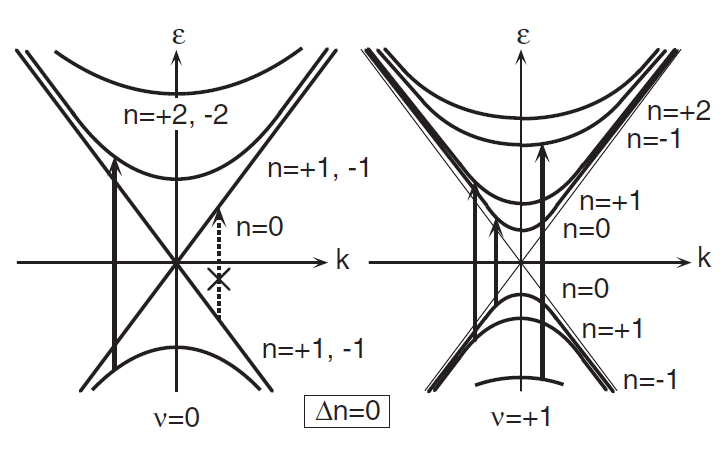
\includegraphics[scale=0.65]{images/chapter_optical_props/selection_rules_1.png}
		\caption{Selection Rules for light polarized parallel to the axial direction of carbon nanotubes. In the $\nu=0$ case, transitions within the Dirac cone are forbidden.}
	\end{subfigure}
	\begin{subfigure}{\textwidth}
		\centering
		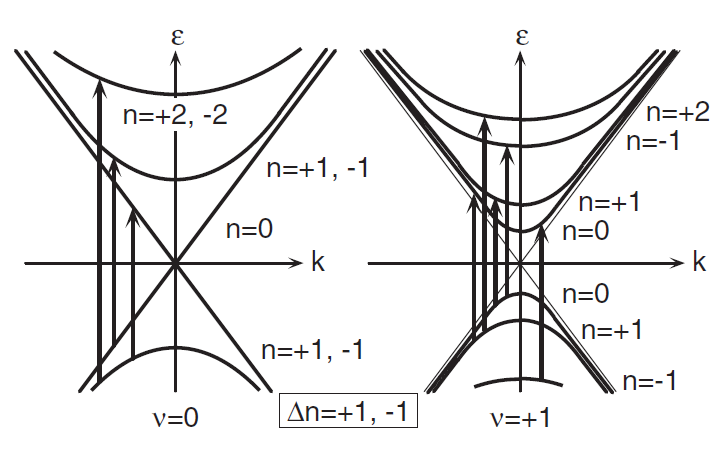
\includegraphics[scale=0.65]{images/chapter_optical_props/selection_rules_2.png}
		\caption{Selection Rules for light polarized perpendicular to the axial direction of carbon nanotubes.}
	\end{subfigure}
	\caption{Optical selection rules for metallic and narrow-gap semiconducting nanotubes ($\nu = 0 $) as well as medium-gap semiconducting nanotubes ($\nu = \pm 1$) . Reproduced from Ref \cite{ando2005theory}.}
	\label{fig:selection_rules}
\end{figure}


 
\subsection{The Effects of Electron-Electron Interactions}

In this simple tight-binding picture, the density of states contains a series of Van-Hove singularities. However, note that tight-binding ignores the effects of electron-electron interactions and thereby does not fully account for the effects of quantum confinement \cite{weismanKonoBook}. Indeed, the inclusion of electron-electron interactions into this picture yields a new electronic structure in which free electrons play a minimal role.

Strong electron-electron interactions influence the binding energies of quasi-particles known as excitons that form after the creation of an electron-hole pair \cite{koch2006semiconductor}. Excitons represent hydrogen-like quasi-particles composed of a negatively-charged electron bound to a positively-charged hole \cite{koch2006semiconductor}. In an ideal 1-D material, theory predicts that excitons will have an infinite binding energy. This alone foreshadows the dominance of excitons in the optical properties of carbon nanotubes \cite{ando2005theory}. 

\begin{figure}[h]
	\centering
	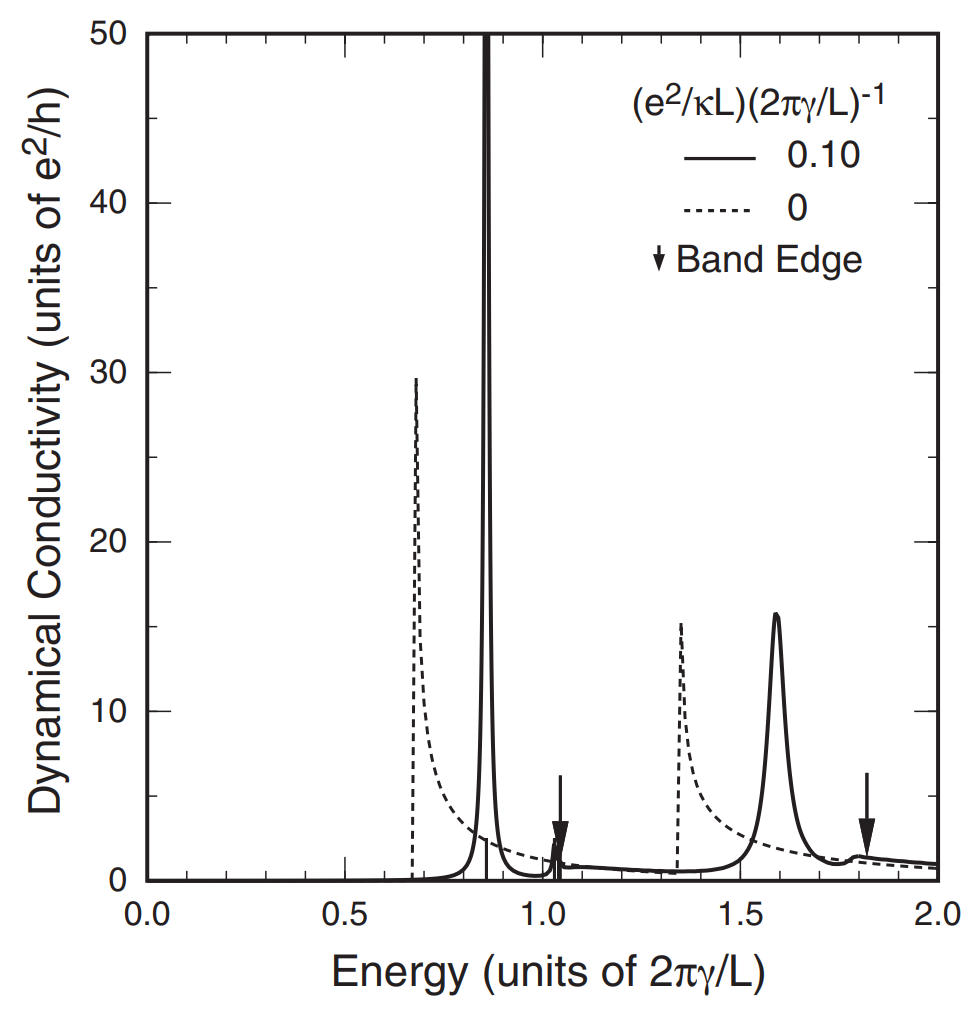
\includegraphics[scale=0.35]{images/chapter_optical_props/ando_suppression}
	\caption{Optical absorption spectrum of a semiconducting nanotube with (solid line) and without (dashed line) the effect of Coulomb interactions. Arrows mark the band edge positions of free electron continua. Reproduced and modified from Ref \cite{ando2005theory}.}
	\label{fig:ando_suppression}
\end{figure}

The strong quantum confinement of nanotubes effectively suppresses the density of states of any free electron continuum whilst enhancing that of excitonic states. Moreover, the effective strength of Coulomb interactions $S_{e-e}$ can be expressed as 
\begin{equation}
	S_{e-e} = \dfrac{e^2 \kappa L}{2 \pi \gamma/L},
\end{equation}

where $e^2 /\kappa L$ and $2 \pi \gamma / L$ account for the characteristic energy scales associated with Coulomb interactions and the kinetic energy of electrons respectively \cite{ando2005theory}. Here, $e$ defines the charge of an electron, $\gamma$ represents a free parameter, $L$ indicates the nanotube circumference $|\vec{C_h}|$, and $\kappa$ denotes the static dielectric constant used to account for screening effects.

Figure \ref{fig:ando_suppression} shows the calculated optical absorption spectrum of a semiconducting nanotube with and without the presence of Coulomb interactions. The plot shows the presence of Van-Hove singularies when ignoring the effect of Coulomb interactions. After accounting for these interactions, the oscillator strength of the low energy bound states of excitons becomes enhanced and absorption in the free-electron continuum drastically diminishes. The band edge of the free-electron continuum also shifts as a result of Coulomb interactions \cite{ando1997excitons}. Furthermore, this shift of the band edge increases as $S_{e-e}$ increases \cite{ando2005theory}. 

\begin{figure}[h]
	\centering
	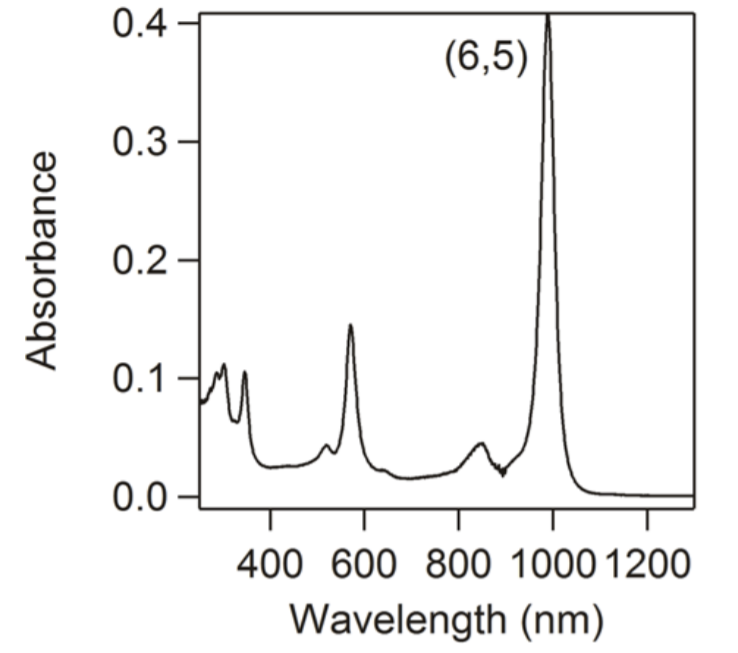
\includegraphics[scale=0.62]{images/chapter_optical_props/cnt_absorbance_yota}
	\caption{Absorbance spectrum of a (6,5) carbon nanotube sample at room temperature. Reproduced from Ref \cite{ichinose2017extraction}. }
	\label{fig:cnt_abs_yota}
\end{figure}

\subsection{Exciton Binding Energies}

The binding energies of excitons in CNTs tend to be on the order of hundreds of meV \cite{wang2005optical}. For instance, the excitons of (6,5) nanotubes have a binding of roughly 400 meV \cite{wang2005optical}. At room temperature $k_b T \approx$ 22 meV, meaning that energy scale associated thermal fluctuations falls short of the exciton binding energies in CNTs. Thus, excitons of CNTs are quite stable at room temperature. Figure \ref{fig:cnt_abs_yota} illustrates this effect as the room-temperature absorbance spectrum of a (6,5) sample exhibits well-defined, excitonic resonances. 

In contrast, conventional semiconductors such as GaAs only exhibit excitons with binding energies typically less than 20 meV \cite{liang1970excitons}.  As a result, these materials have to be cooled down to low temperatures in order to easily observe exciton resonances as shown in Figure \ref{fig:gaas_vs_cnt_absorbance}. 

\begin{figure}[h]
	\centering
	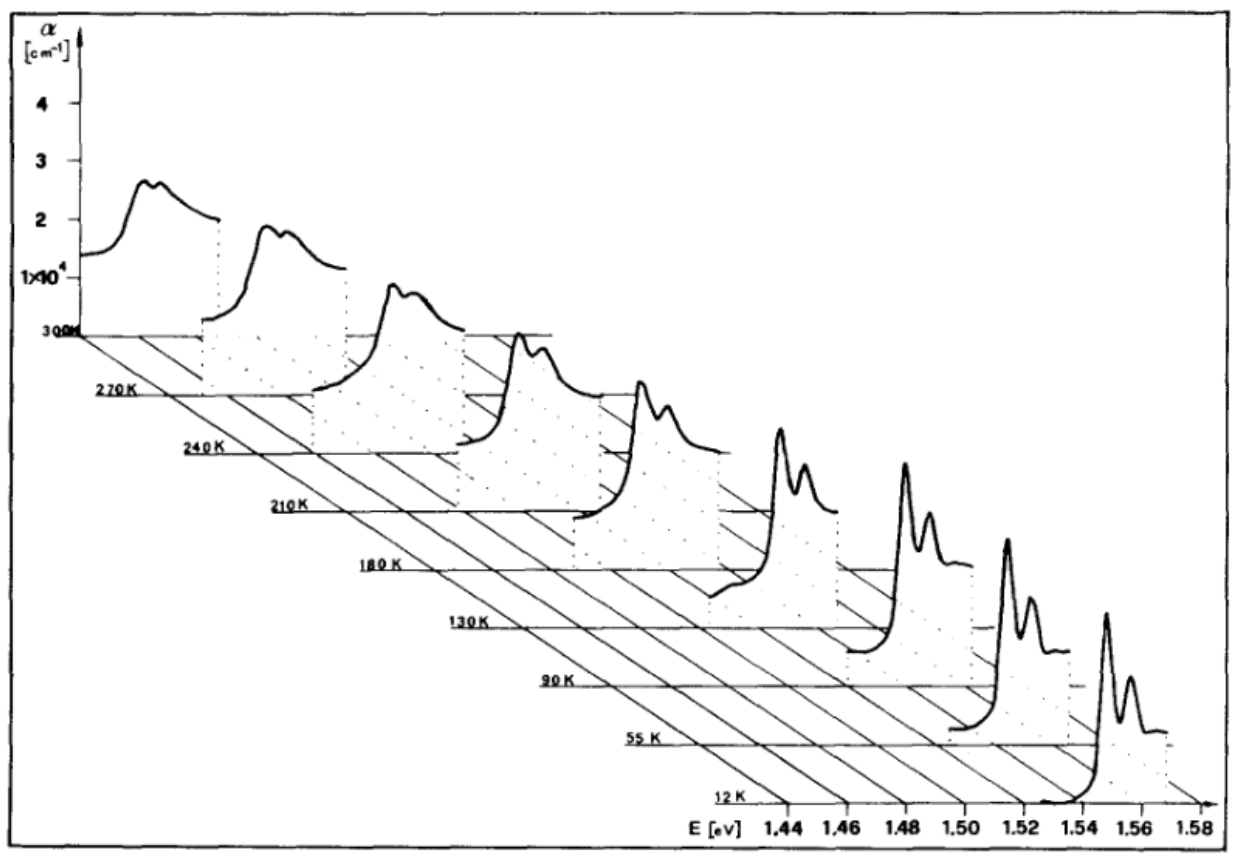
\includegraphics[scale=0.55]{images/chapter_optical_props/gaas_absorbance_filipowicz}
	\caption{Figure of GaAs absorbance at low-T and high-T to show weak binding energy of excitons. Reproduced from Ref \cite{filipowicz1990temperature}.}
	\label{fig:gaas_vs_cnt_absorbance}
\end{figure}

Figure \ref{fig:gaas_vs_cnt_absorbance} shows the absorption spectrum of GaAs compared with CNTs. GaAs at room temperature does not exhibit any exciton resonance. Must cool down to temperatures as low as 4 K to see sharp exciton resonances. As cool down, linewidths become narrow, indicating that exciton lifetimes increase. However, in CNTs these resonances easily observed at room temperature. 


\section{Summary}

Different species are distinguishable using a set of indices (m,n). Can distinguish between metallic and semiconducting nanotubes with this definition. 1-D character of nanotubes establishes strong quantum confinement, bolsters the role of electron-electron interactions. Strong coulomb interactions lead to excitons with very high binding energies. Theory also shows that excitonic resonances diminish the density of states associated with the free electron continuum. 